\documentclass[12pt]{article}
\usepackage{enumerate}
\usepackage{mathematics}

\DeclareMathOperator{\diam}{\mathrm{diam}}


\begin{document}

\title{Oxford A2 - Metric Spaces and Complex Analysis
  \footnotetext{\url{https://courses.maths.ox.ac.uk/node/5378}}} \author{Dan Davison}
\author{}
\date{}
\maketitle

\section{Sheet 1}

\subsection{}
\begin{mdframed}
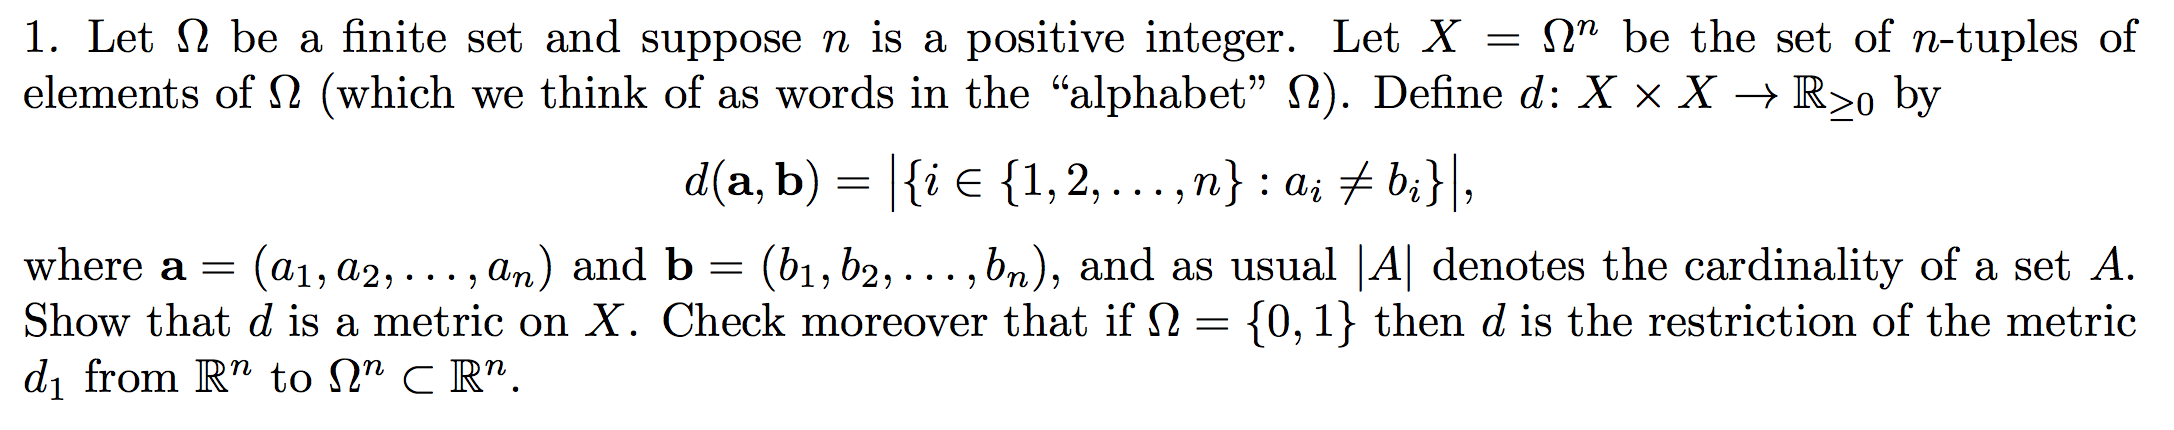
\includegraphics[width=400pt]{img/oxford-a2-1-1.png}
\end{mdframed}

\begin{remark*}
  $d$ is the Hamming distance.
\end{remark*}

For $d$ to be a metric on $X$ we require
\begin{enumerate}
\item \textbf{$d$ is a function $d:X \times X \to $ (a set of non-negative numbers).}\\
  Yes, this is true.
\item \textbf{Positivity}:\\
  Yes, cardinality is never negative and it is clear that $d(a,b) = 0 \iff a = b$.
\item \textbf{Symmetry}:\\
  Yes, follows from the fact that $a_i \neq b_i \iff b_i \neq a_i$.
\item \textbf{Triangle inequality}:\\
  % Want: $d(a, b) \leq d(a, c) + d(c, b)$ for all $a, b, c \in X$.
  Note that $d(a, b) = \sum_{i=1}^n \epsilon_{a_i,b_i}$, where $\epsilon_{ij} :=
  \begin{cases}
    0, ~~~ i = j\\
    1, ~~~ i \neq j
  \end{cases}
$ (the ``negation'' of the Kronecker delta).

  Fix $i \in \{1, 2, \ldots, n\}$. Suppose that $\epsilon_{a_i,b_i} = 0$. Then
  $\epsilon_{a_i,b_i} \leq \epsilon_{a_i,c_i} + \epsilon_{c_i,b_i}$. Alternatively suppose that
  $\epsilon_{a_i,b_i} = 1$. Then we have either $\epsilon_{a_i,c_i} = 0$, in which case
  $\epsilon_{c_i,b_i} = \epsilon_{a_i,b_i} = 1$, or we have $\epsilon_{a_i,c_i} = 1$.

  Therefore $\epsilon_{a_i,b_i} \leq \epsilon_{a_i,c_i} + \epsilon_{c_i,b_i}$, and therefore
  $\sumin \epsilon_{a_i,b_i} \leq \sumin \epsilon_{a_i,c_i} + \sumin \epsilon_{c_i,b_i}$, as required.
\end{enumerate}

Recall that $d_1:\R^n\times\R^n\to\R_{\geq 0}$ is given by $d_1(a, b) := \sum_{i=1}^n|a_i - b_i|$.

Let $\Omega = \{0, 1\} \subseteq \R$ and let $a, b \in \Omega^n \subseteq \R^n$.

Note that $|a_i - b_i| = \epsilon_{a_ib_i}$.

Therefore $d_1(a, b) = \sum_{i=1}^n\epsilon_{a_ib_i} = d(a, b)$, as required.

\newpage
\subsection{}
\begin{mdframed}
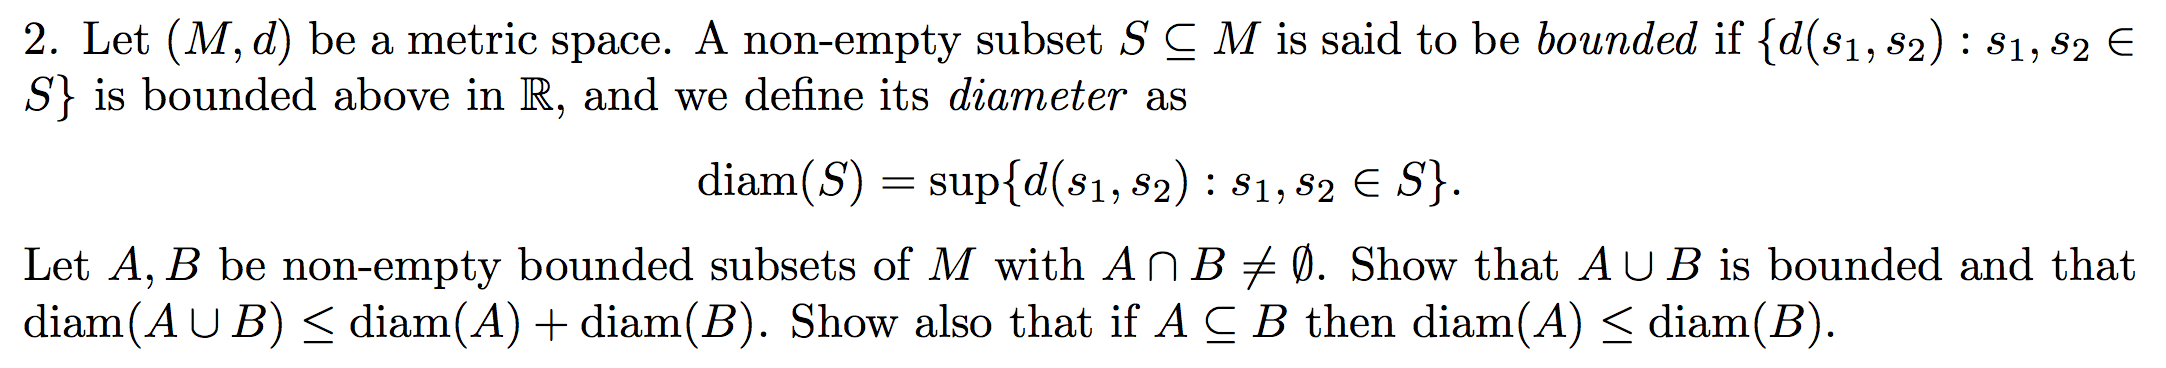
\includegraphics[width=400pt]{img/oxford-a2-1-2.png}
\end{mdframed}

\begin{claim*}
  $A \cup B$ is bounded and $\diam(A \cup B) \leq \diam(A) + \diam(B)$.
\end{claim*}

\begin{proof}
  Let $c_1, c_2 \in A \cup B$.

  Note that $c_1, c_2 \in A \implies d(c_1, c_2) \leq \diam(A)$ and
  $c_1, c_2 \in B \implies d(c_1, c_2) \leq \diam(B)$.

  Suppose, without loss of generality, that $c_1 \in A$ and $c_2 \in B$. Let $c_3 \in A \cap
  B$. Then by the triangle inequality we have
  $d(c_1, c_2) \leq d(c_1, c_3) + d(c_3, c_2) \leq \diam(A) + \diam(B)$.

  Therefore $A \cup B$ is bounded and $\diam(A \cup B) \leq \diam(A) + \diam(B)$.
\end{proof}


\begin{claim*}
  If $A \subseteq B$ then $\diam(A) \leq \diam(B)$.
\end{claim*}

\begin{proof}
  Let $A \subseteq B$, and suppose for a contradiction that $\diam(A) > \diam(B)$. Then there exist
  $a_1, a_2 \in A$ such that $d(a_1, a_2) > \diam(B)$. But since $A \subseteq B$ we have
  $a_1, a_2 \in B$. This contradicts the definition of $\diam(B)$ as the supremum over distances
  between pairs of elements of $B$. Therefore $\diam(A) \leq \diam(B)$.
\end{proof}


\newpage
\subsection{}
\begin{mdframed}
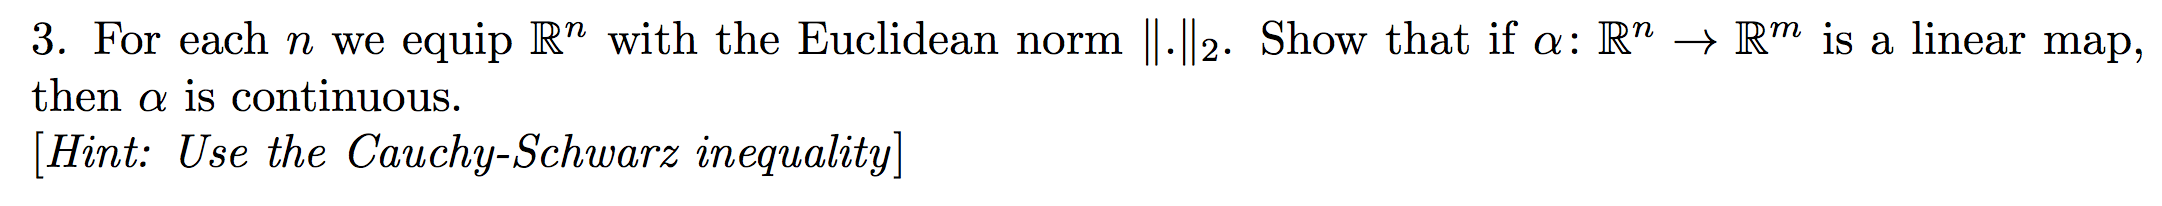
\includegraphics[width=400pt]{img/oxford-a2-1-3.png}
\end{mdframed}

\begin{lemma*}
  Let $f:V \to W$ be a linear map between normed vector spaces. Then $f$ is continuous if and only
  if $\{\norm{f(x)} : \norm{x} \leq 1\}$ is bounded.
\end{lemma*}

\begin{proof}
  See $\epsilon-\delta$ argument in lecture notes.
\end{proof}

% \begin{claim*}
%   The Euclidean norm is independent of basis.
% \end{claim*}

% \begin{proof}~\\
%   Let $B$ and $B'$ be bases of $\R^n$ and let $P$ be a matrix with the elements of $B'$ as its
%   columns.

%   I.e. if $v$ contains the coordinates of a vector with respect to basis $B$, Then $Pv$...

%   With respect to $B$, we have $\norm{v} = \sqrt{\sumin v_i^2}$.

%   With respect to $B'$, we have $\norm{v} = \sqrt{\sumin (Pv_i)^2}$.
% \end{proof}

\begin{claim*}
  $\{\norm{\alpha(x)} : \norm{x} \leq 1\}$ is bounded. \Intuition{the image of the unit sphere is
    bounded in norm}
\end{claim*}

\begin{proof}
  Note that $\norm{\alpha(x)}^2 := \sum_{i=1}^n \alpha(x)_i^2$, where $\alpha(x)_i$ is the $i$-th
  coordinate of $\alpha(x)$ with respect to the standard basis.

Therefore it is sufficient to show that $\{|\alpha(x)_i| : \norm{x} \leq 1\}$ is bounded for all
$1 \leq i \leq n$.

Let $a_i$ be the $i$-th row of the $m \times n$ matrix of $\alpha$.

Then $|\alpha(x)_i| = |\langle a_i, x \rangle| \leq \norm{a_i}\norm{x}$.
\end{proof}

% \begin{intuition*}
%   The proof of the (linear, continuous) $\iff$ (linear, image bounded in norm) lemma uses
%   $\epsilon-\delta$ arguments. Then we use Cauchy-Schwarz to show that the image of the unit
%   sphere is bounded in norm as prescribed.
% \end{intuition*}

\newpage
\subsection{}
\begin{mdframed}
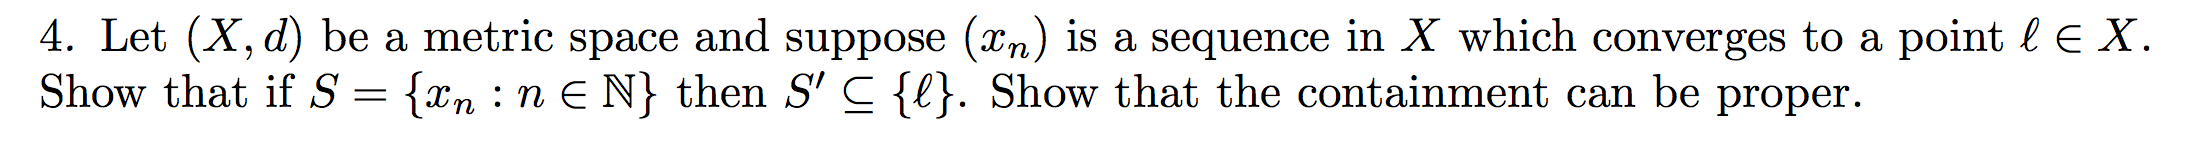
\includegraphics[width=400pt]{img/oxford-a2-1-4.png}
\end{mdframed}

\begin{proof}~\\
  Let $B(x, r)$ be an open ball of radius $r$ centered at $x$.

  Note that for every $\delta > 0$ there exists $N \in \N$ such that $d(x_n, \ell) < \delta$ for all
  $n > N$.

  Let $y \neq \ell$ and let $N = \min\{n ~|~ d(x_n, \ell) < d(y, \ell)\}$.

  Let $M = \argmin_{n \in \{1, \ldots, N\}} D(n)$, where $D:\N \to \R$ is defined by
  $D(n) :=
  \begin{cases}
    d(x_n, y), &x_n \neq y\\
    \infty, &x_n = y
  \end{cases}$.

  Informally, $x_M$ is the element of $S$ that is closest but not equal to $y$.

  Note that $\Big(B(\ell, \frac{x_M - y}{2})\setminus\{\ell\}\Big) \cap S = \emptyset$.

  Therefore $y \neq \ell \implies y \notin S'$, or equivalently, $S' \seq \{\ell\}$.

  Now suppose that $S$ is such that there exists $N \in \N$ such that $x_n = \ell$ for all $n > N$.

  Let $M = \max\{n ~|~ x_n \neq \ell\}$.

  Note that $\Big(B(\ell, \frac{x_M - \ell}{2})\setminus\{\ell\}\Big) \cap S = \emptyset$.

  Therefore it is possible that $\ell \notin S'$, or equivalently, $S' = \emptyset$.
\end{proof}

\newpage
\begin{mdframed}
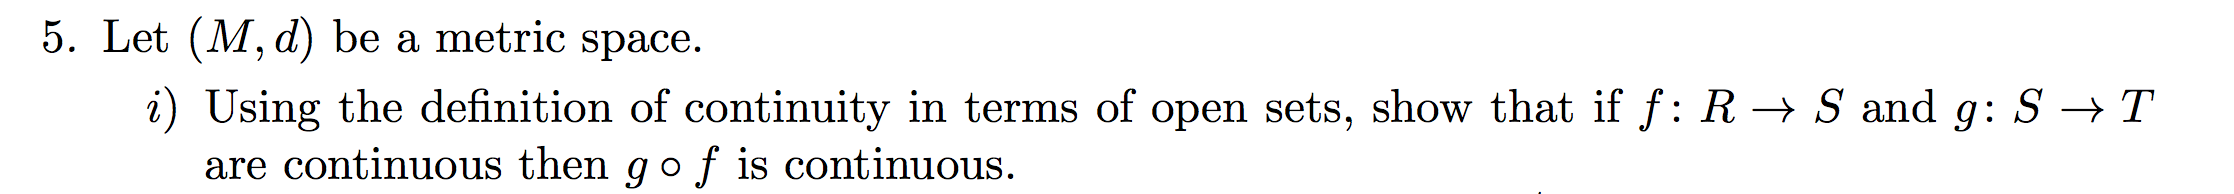
\includegraphics[width=400pt]{img/oxford-a2-1-5-1.png}
\end{mdframed}

\begin{lemma*}
  Let $X$ and $Y$ be metric spaces. $h:X \to Y$ is continuous iff for every open set $U \in Y$, the
  preimage $h^\1(U)$ is an open set in $X$.
\end{lemma*}

\begin{claim*}
  $(g \circ f):R \to T$ is continuous.
\end{claim*}

\begin{proof}
Let $U_T$ be an open set of $T$.

Note that $(g \circ f)^\1(t) = f^\1(g^\1(t))$.

By the lemma, since $f$ and $g$ are continuous, $f^\1(g^\1(U_T))$ is an open set in $R$.
\end{proof}

\begin{mdframed}
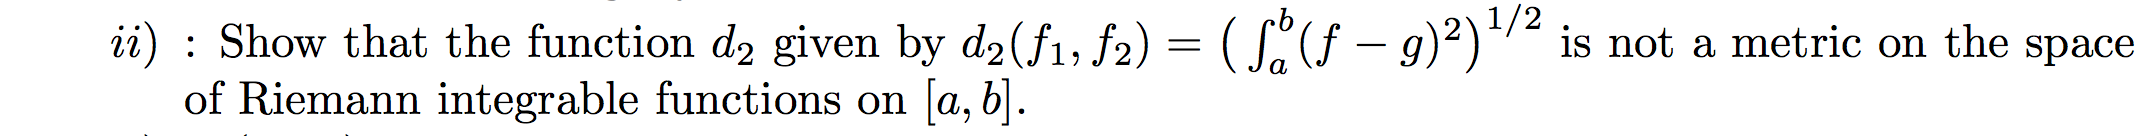
\includegraphics[width=400pt]{img/oxford-a2-1-5-2.png}
\end{mdframed}

Where does it fail?

\begin{enumerate}
\item Positivity?
\item Symmetry?
\item Triangle inequality?
\end{enumerate}

\begin{mdframed}

\includegraphics[width=400pt]{img/oxford-a2-1-5-3.png}
\end{mdframed}

\begin{definition*}
  A subset $X \seq M$ is open if at every point $x \in X$ there exists a $\delta$ such that
  $B(x, \delta) \seq X$.
\end{definition*}

\begin{proof}~\\
  If $M$ is empty it is vacuously true, so suppose $M$ is not empty.

  $M$ itself is open since there are no points outside $M$, so any ball centred on a point of $M$
  must be a subset of $M$.

  Suppose that $X \subset (M, d)$ is not open.

  Then there exists $x \in X$ with the following property: there does not exist $\delta > 0$ such
  that $B(x, \delta) \seq X$.

  However, $M$ is finite. Therefore we may pick the element of $M$ that is closest to $x$, and set
  $\delta$ to be half this distance.

  This contradiction shows that no such non-open $X$ exists.
\end{proof}

\begin{mdframed}
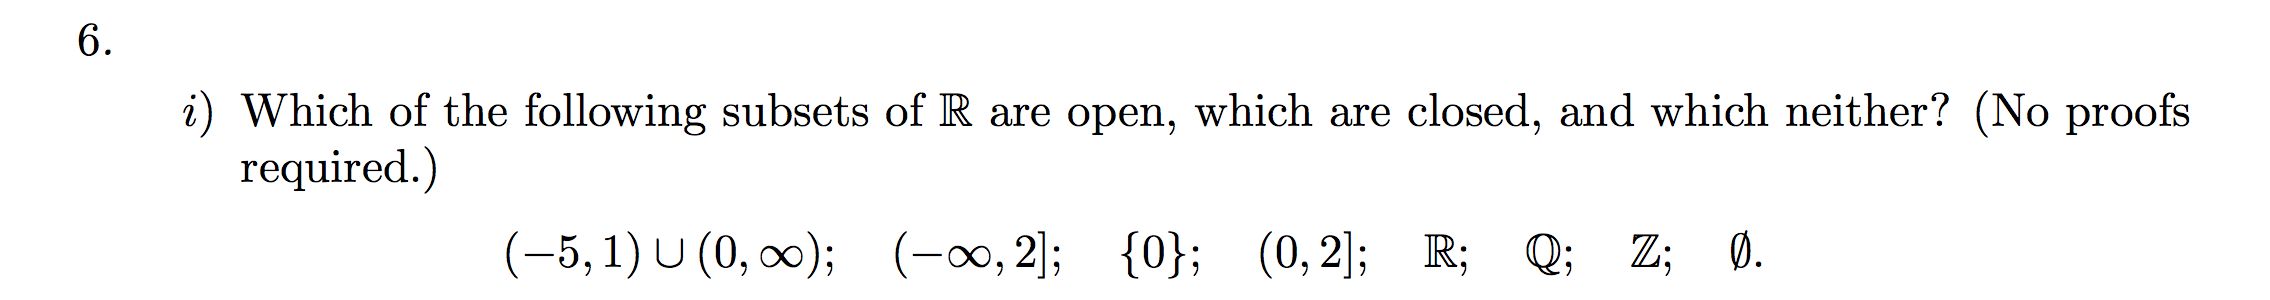
\includegraphics[width=400pt]{img/oxford-a2-1-6-1.png}
\end{mdframed}

\begin{enumerate}
\item $(-5, 1) \cup (0, \infty) = (-5, \infty)$ open, not closed
\item $(-\infty, 2]$ not open, closed
\item $\{0\}$ not open, closed
\item $(0, 2]$ not open, not closed
\item $\R$ open, closed
\item $\Q$ not open, not closed (any interval $I \seq \R$ contains both rationals and irrationals)
\item $\Z$ not open, closed
\item $\emptyset$ open, closed
\end{enumerate}

\begin{mdframed}
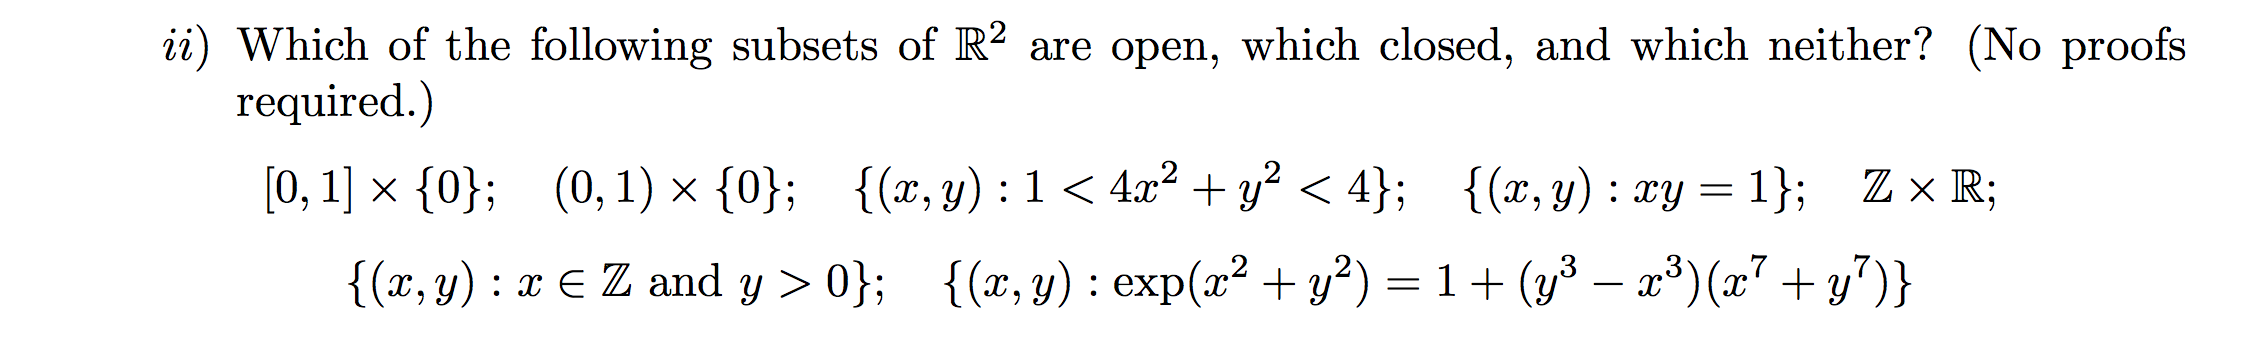
\includegraphics[width=400pt]{img/oxford-a2-1-6-2.png}
\end{mdframed}

\begin{enumerate}
\item $[0, 1] \times \{0\}$ not open, closed\\
  \begin{tiny}
    A ball at any point will contain points outside, so not open.\\
    Complement is open, so closed.
    \par
  \end{tiny}
\item $(0, 1) \times \{0\}$ not open, not closed\\
  \begin{tiny}
    A ball at any point will contain points outside (by poking out in the y direction), so not open.\\
    Complement is not open (e.g. contains origin)
    \par
  \end{tiny}
\item $\{(x,y) ~|~ 1 < 4x^2 + y^2 < 4\}$ open, not closed\\
  {\tiny
    Region sandwiched between inner and outer ellipse.\\
    Clearly open, complement not open.
    \par}
\item $\{(x,y) ~|~ xy = 1\}$ not open, closed\\
  {\tiny
    clearly not open, e.g. ball at $(1,1)$ leaves the set\\
    complement is open
    \par}
\item $\Z \times \R$ not open, closed\\
  {\tiny
    Collection of horizontal lines.\\
    Not open, any ball will poke up/down in the y-direction, leaving the set.\\
    Complement is $\R^2$ with a collection of horizontal lines deleted.\\
    So complement is open.
    \par}
\item $\{(x,y) ~|~ x \in \Z \text{~and~} y > 0\}$ not open, not closed\\
  {\tiny
    Vertical lines, starting just above the y=0 line.\\
    Clearly not open.\\
    Complement not open, since it includes the y=0 line.
    \par}
\item $\{(x,y) ~|~ \exp(x^2 + y^2) = 1 + (y^3 - x^3)(x^7 + y^7)\}$ not open, closed\\
  \begin{tiny}
    One equation in 2D ambient space $\implies$ no solutions or a line of solutions.\\
    0 is a solution $\implies$ line of solutions $\implies$ not open, closed.\\
    \par
  \end{tiny}
\end{enumerate}

\newpage
\begin{mdframed}
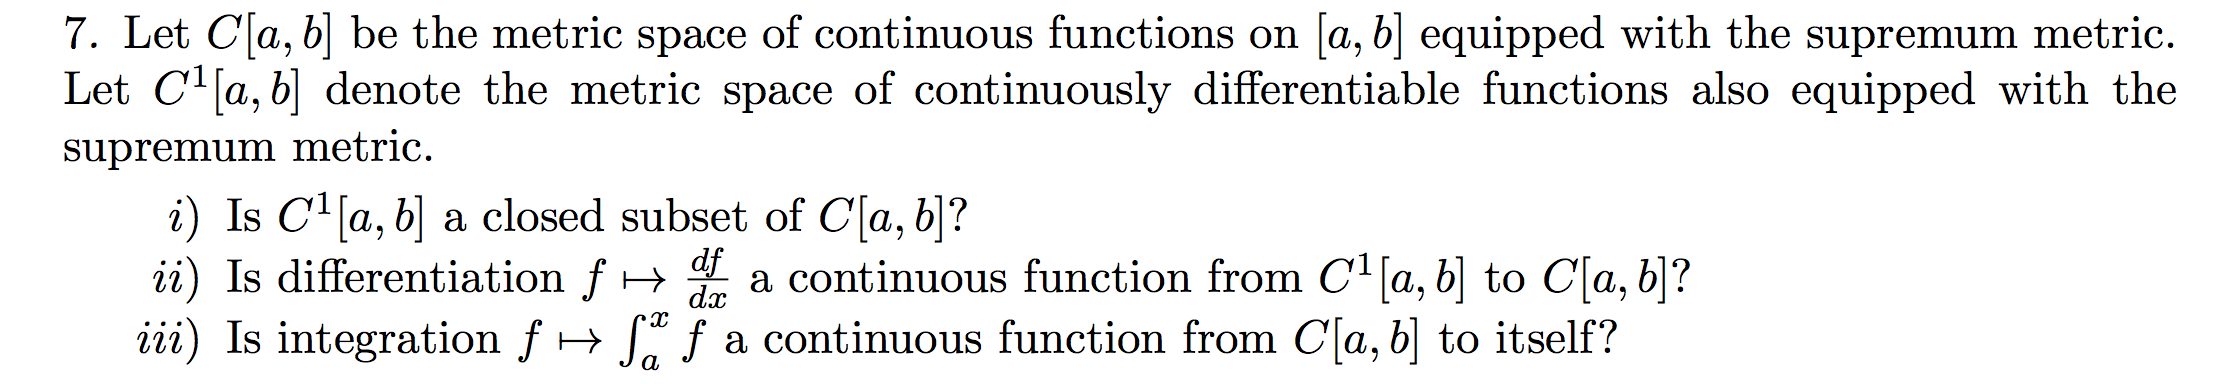
\includegraphics[width=400pt]{img/oxford-a2-1-7.png}
\end{mdframed}

% \begin{remark*}
%   Since on a closed interval every continuous function is bounded and attains its bounds, the
%   supremum metric here is just a max metric.
% \end{remark*}

\begin{mdframed}
\begin{lemma*}
  Let $f:V \to W$ be a linear map between normed vector spaces. Then $f$ is continuous if and only
  if $\{\norm{f(v)} : \norm{v} \leq 1 \}$ is bounded.
\end{lemma*}

\begin{proof}
  See question 3.
\end{proof}
\end{mdframed}

% \url{https://math.stackexchange.com/questions/975759/are-differentiation-and-integration-continuous-functions}

\begin{enumerate}[label=\roman*)]
\item \textbf{Is $C^1[a,b]$ a closed subset of $C[a,b]$?}
  \red{TODO}

  $C^1[a,b] \seq C[a, b]$ is closed iff its complement is open.

  To answer this question we can either show that its complement is not open (could be done by
  counter-example), or open (requires positive proof).

  The complement of $C^1[a,b] \seq C[a, b]$ is the set of continuous functions that are not
  continuously differentiable. An example is $x \mapsto |x|$.

  Counter-example approach: if we could exhibit a pair of functions $f \in (C^1[a,b])^C$ and
  $g \in C^1[a,b]$, such that the distance between $f$ and $g$ can be made arbitrarily small, then
  this would prove that $(C^1[a,b])^C$ is not open and hence that $C^1[a,b]$ is not a closed subset
  of $C[a,b]$.

% \item Let $f,g \in C^1[a,b]$, let $h = f - g$ and fix $\epsilon > 0$.

%   For continuity at $f$ we seek $\delta > 0$ such that
%   \begin{align*}
%     & \sup_{x \in [a,b]} |f(x) - g(x)| < \delta \implies \sup_{x \in [a,b]} |f'(x) - g'(x)| < \epsilon\\
%     \iff & \sup_{x \in [a,b]} |(f - g)(x)| < \delta \implies \sup_{x \in [a,b]} |(f - g)'(x)| < \epsilon\\
%     \iff & \sup_{x \in [a,b]} |h(x)| < \delta \implies \sup_{x \in [a,b]} |h'(x)| < \epsilon.
%   \end{align*}
%   Suppose that such a $\delta$ exists.

\newpage
\item \textbf{Is differentiation continuous?}\\

  \begin{proof} (I)~\\
    Let $C[a,b]$ be the metric space of continuous functions on $[a,b]$ equipped with the supremum
    metric.

    Let $C^1[a,b]$ be the metric space of continuously differentiable functions on $[a,b]$ also
    equipped with the supremum metric.

    Note that the differentiation operator $D:C^1[a,b] \to C[a,b]$ is a linear map between vector
    spaces.

    Define a norm on $C[a,b]$ by $\norm{f} := \sup_{x\in [a,b]}|f(x)|$.

    Then, according to the lemma, $D$ is continuous if and only if
    $\{\norm{D(f)} : \norm{f} \leq 1 \}$ is bounded.

    Suppose for a contradiction that $M$ is such a bound.

    But consider the logistic function $f:[a,b] \to (0, 1)$ given by
    $f(x) := (1 + e^{-4(M+1)(x-a)})^{-1}$.

    Clearly $\norm{f} < 1$.

    Its derivative is $f'(x) = 4(M+1)f(x-a)(1-f(x-a))$ which (I assert) is continuous.

    So we have $f \in C^1[a,b]$ and $\norm{f} < 1$ and yet $f'(a) = M+1$.

    Therefore no such bound $M$ exists. Therefore the differentiation operator is not continuous.
  \end{proof}

  \begin{proof} (II Alex Coward)~\\
    Define $D:C^1[a,b] \to C[a,b]$ to be differentiation.

    We construct a sequence of functions that tend to the zero function, but whose derivatives
    always have image $[0, 1]$.

    Define $f_n(x) := \frac{1}{n}\sin\(\frac{nb}{2\pi}(x - a)\)$.

    Note that $(D f_n)(x) = \frac{b}{2\pi}\cos\(\frac{nb}{2\pi}(x - a)\)$.

    Note also that $\limn f_n = 0$.

    Suppose for a contradiction that $D$ is continuous.

    Then $\limn D(f_n) = D(\limn f_n) = D(0) = 0$.


  \end{proof}

\newpage
\item \textbf{Is integration continuous?}\\
  Let $C[a,b]$ be the metric space of continuous functions on $[a,b]$ equipped with the supremum
  metric.

  Let $C^1[a,b]$ be the metric space of continuously differentiable functions on $[a,b]$ also
  equipped with the supremum metric.

  Note that the integration operator defined by $F(f) := \int_a^x f$ is a linear map between vector
  spaces.

  Define a norm on $C[a,b]$ as $\norm{f} := \sup_{x\in [a,b]}|f(x)|$.

  Then, according to the lemma, $F$ is continuous if and only if
  $\{\norm{F(f)} : \norm{f} \leq 1 \}$ is bounded.

  Note that on a closed interval every continuous function is bounded.

  Let $f \in C[a,b]$ and let $L$ and $M$ be the lower and upper bounds of $f$ respectively.

  Then $(F(f))(x) \leq (M-L)x$, for all $x \in [a,b]$.

  Therefore $F$ is continuous.

\end{enumerate}

\newpage
\begin{mdframed}
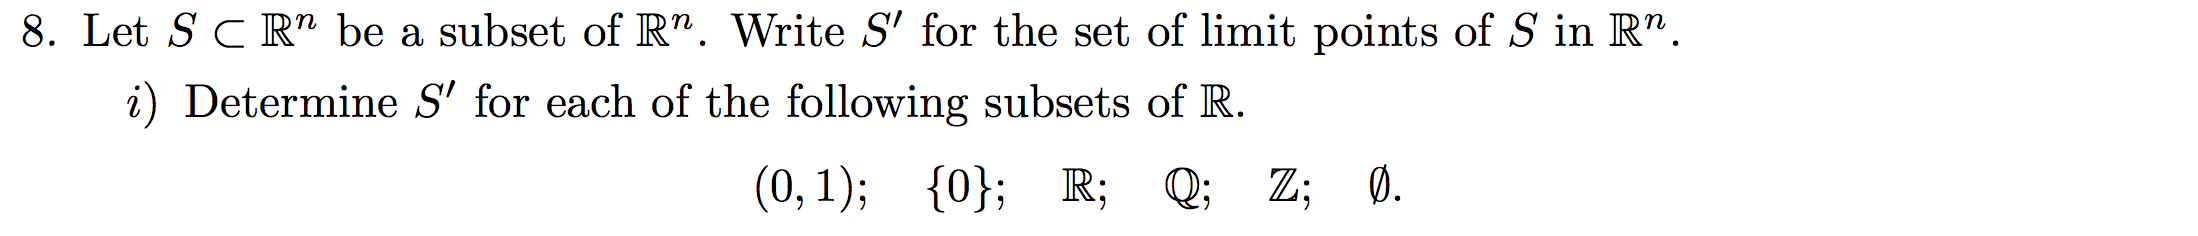
\includegraphics[width=400pt]{img/oxford-a2-1-8-1.png}
\end{mdframed}

\begin{table}[h!]
  \begin{tabular}{c|c|l}
    $S$         &$S'$         &                \\
    \hline
    $(0, 1)$    & $[0, 1]$    &                \\
    $\{0\}$     & $\emptyset$ & 0 is an isolated point \\
    $\R$        & $\R$        &                \\
    $\Q$        & $\Q$        & Any ball placed on a rational contains both other rationals and irrationals.\\
    $\Z$        & $\emptyset$ & All integers are isolated points.               \\
    $\emptyset$ & $\emptyset$ &
  \end{tabular}
\end{table}

\begin{mdframed}

\includegraphics[width=400pt]{img/oxford-a2-1-8-2.png}
\end{mdframed}

% \begin{proof}~\\
%   Let $S \subset \R$.

%   Let $u \in (S')'$.

%   Then $\Big(B(u, \epsilon) \setminus \{u\}\Big) \cap S' \neq \emptyset$ for all $\epsilon > 0$.

%   Therefore there exists $t \in (S')'$ such that $t \in S'$.

%   If $t \in S$

%   Want: $\Big(B(u, \epsilon) \setminus \{u\}\Big) \cap S \neq \emptyset$ for all $\epsilon > 0$.
% \end{proof}

\begin{mdframed}
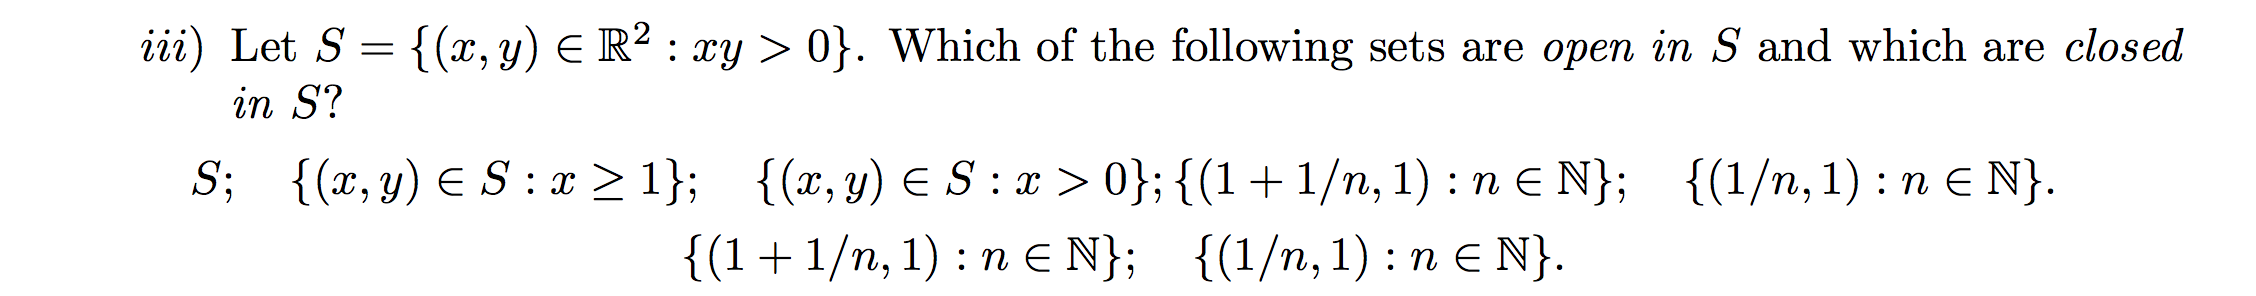
\includegraphics[width=400pt]{img/oxford-a2-1-8-3.png}
\end{mdframed}

\begin{table}[h!]
  \begin{tabular}{l|c|l|l}
    $S$                                 &  open          &   closed      &    \\
    $\{(x, y) \in S ~|~ x \geq 1\}$     &  open          &   closed      &    \\
    $\{(x, y) \in S ~|~ x > 0\}$        &  not open      &   open        &    \\
    $\{(1 + 1/n, 1) ~|~ n \in \N\}$     &  not open      &   not closed  & complement contains $(1,1)$   \\
    $\{(1/n, 1) ~|~ n \in \N\}$         &  not open      &   closed      & unlike previous, complement excludes $(0, 0)$\\
  \end{tabular}
\end{table}


% \newpage

\begin{mdframed}
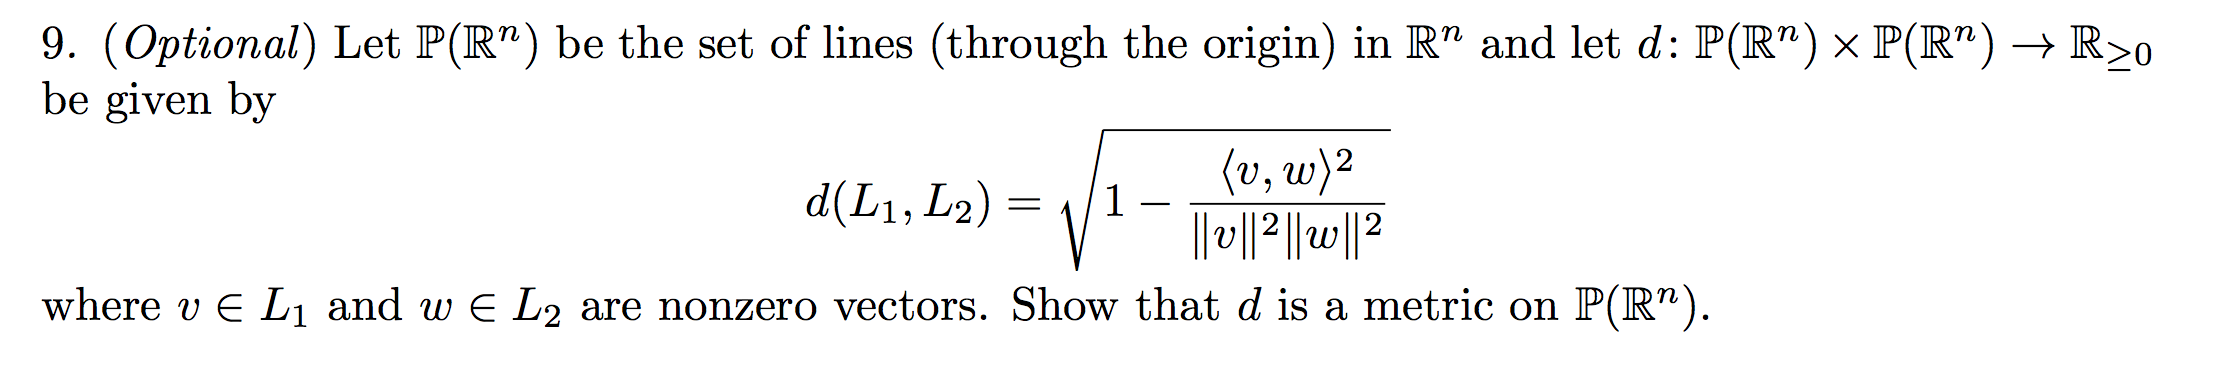
\includegraphics[width=400pt]{img/oxford-a2-1-9.png}
\end{mdframed}

\begin{proof}~\\
  \textbf{Well-defined:}

  \textbf{Positivity}: By Cauchy-Schwartz, for non-zero $v, w$, we have
  \begin{align*}
    0 < ~&\frac{\langle v, w \rangle}{\norm{v}\norm{w}} \leq 1\\
    0 \leq~ &1 - \(\frac{\langle v,w\rangle}{\norm{v}\norm{w}}\)^2 < 1\\
    0 \leq~ &d(L_1, L_2) < 1
  \end{align*}
  (since we take the positive square root).

  \textbf{Symmetry}:

\end{proof}


\section{Sheet 2}


\subsection{}
\begin{mdframed}
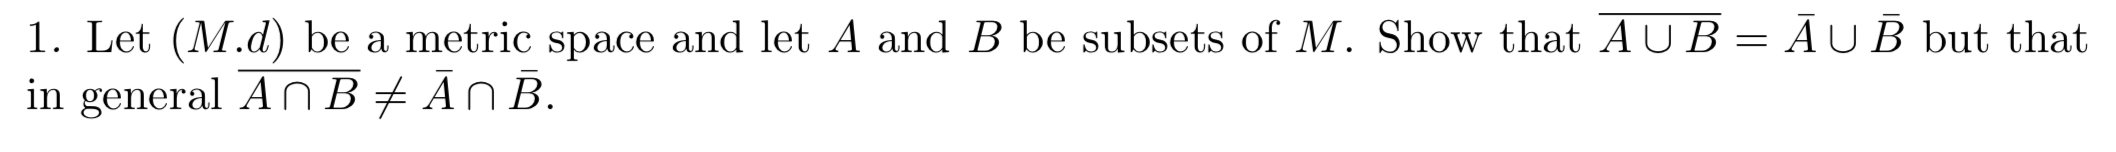
\includegraphics[width=400pt]{img/oxford-a2-2-1.png}
\end{mdframed}

Let $(M, d)$ be a metric space and let $A, B \subseteq M$.

\red{Incomplete}

\begin{claim*}
  $\bar{A \cup B} = \bar A \cup \bar B$.
\end{claim*}
\begin{proof}~\\
  {\bf Forward inclusion}\\
  Let $x \in \bar{A \cup B}$. Then either $x \in A \cup B$ or $x$ is a limit point, but not a
  member, of $A \cup B$.

  If $x \in A \cup B$ then either $x \in A$ (in which case $x \in \bar A$) or $x \in B$ (in which
  case $x \in \bar B$): in both cases we have $x \in \bar A \cup \bar B$.

  Alternatively, suppose $x \in (A \cup B)'$ and $x \notin A \cup B$. Then for all $\epsilon > 0$
  we have that either $B(x, \epsilon) \cap A \neq \emptyset$ or
  $B(x, \epsilon) \cap B \neq \emptyset$. Therefore $x$ is a limit point of either $A$ or $B$. (To
  see this, WLOG suppose there exists $\phi > 0$ such that for all $0 < \epsilon < \phi$ we have
  $B(x, \epsilon) \cap A = \emptyset$. Then for all $0 < \epsilon < \phi$ we have
  $B(x, \epsilon) \cap B \neq \emptyset$ and $x$ is a limit point of $B$. Alternatively, $x$ is a
  limit point of both $A$ and $B$.) Therefore either $x \in \bar A$ or $x \in \bar B$ as required.

  {\bf Reverse inclusion}\\
  Let $x \in \bar A \cup \bar B$. WLOG let $x \in \bar A$. Then either $x \in A$ or $x$ is a limit
  point, but not a member, of $A$.

  If $x \in A$ then $x \in \bar A \subseteq \bar{A \cup B}$, and so $x \in \bar{A \cup B}$ as
  required.

  Alternatively, suppose $x$ is a limit point, but not a member, of $A$. Then $x$ is a limit point
  of $A \cup B$ and so $x \in \bar{A \cup B}$ as required.
\end{proof}

\begin{claim*}
  $\bar{A \cap B} \neq \bar A \cap \bar B$.
\end{claim*}
\begin{proof}
  \red{TODO}
\end{proof}

\newpage
\subsection{}



\begin{mdframed}
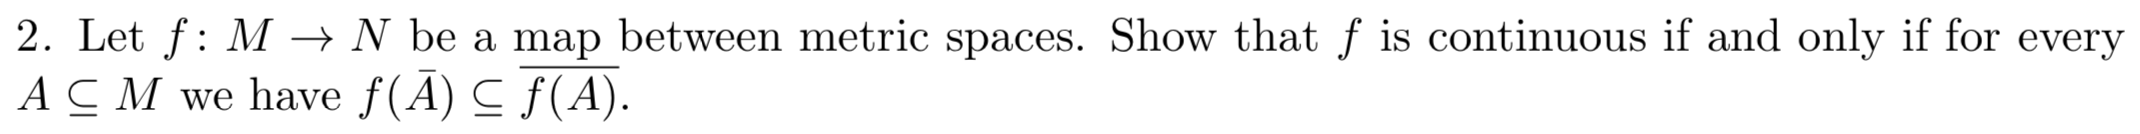
\includegraphics[width=400pt]{img/oxford-a2-2-2.png}
\end{mdframed}

\begin{mdframed}
\begin{intuition*}
  This claim is saying that $f$ is continuous iff for all subsets $A \subseteq M$, the external
  limit points of $A$ remain close to points of $A$ when forming the image under $f$.

  So the forward implication is unsurprising: continuity keeps them close.

  Regarding the reverse implication, if they remain close for all subsets $A$ then this ``remaining
  close'' is occurring across the whole of $M$, so it is plausible that this means $f$ is
  continuous.
\end{intuition*}
\end{mdframed}

\begin{claim*}
  Let $f:M \to N$ be a map between metric spaces. Then $f$ is continuous if and only if for every
  $A \subseteq M$ we have $f(\bar A) \subseteq \bar{f(A)}$.
\end{claim*}

\begin{proof}
  Let $f:M \to N$ be a map between metric spaces.

  $\implies$\\
  Suppose $f$ is continuous and let $A \subseteq M$. Note that $f^\1(\bar{f(A)})$ is closed (by
  continuity of $f$) and contains $A$. Therefore\footnote{Let $X, Y$ be subsets of a metric
    space. If $Y$ is closed and $X \subseteq Y$ then $\bar X \subseteq Y$.}
  $\bar A \in f^\1(\bar{f(A)})$. Therefore $f(\bar A) \in \bar{f(A)}$.

  $\impliedby$\\
  Suppose that for every $A \subseteq M$ we have $f(\bar A) \subseteq \bar{f(A)}$.

  We will show that for every closed $B \subseteq N$ we have that $f^\1(B)$ is closed.

  So let $B \subseteq N$ be closed and let $A = f^\1(B)$.

  Then $f(A) \subseteq B$ and since $B$ is closed, $\bar{f(A)} \subseteq B$ and therefore
  $f(\bar A) \subseteq \bar{f(A)} \subseteq B$.

  So we have $f(\bar A) \subseteq B$ or equivalently $\bar A \subseteq f^\1(B) = A$.

  Therefore $\bar A = A$ and so $A$ is closed.
\end{proof}

\blue{Alternative proof of forward implication using convergent sequences (can reverse implication
  be done in a related way?)}

{\bf Notation.} $A'$ denotes the set of limit points of $A$.

\begin{lemma}\label{external-limit-points-suffice}
  Let $f:M \to N$ be a map between metric spaces and let $A \subseteq M$. Then
  \begin{align*}
    f(\bar A) \subseteq \bar{f(A)} \iff f(A' \setminus A) \subseteq \bar{f(A)}.
  \end{align*}
\end{lemma}
\begin{proof}~\\
  Note that $\bar A = A \cup (A' \setminus A)$, therefore
  $f(\bar A) = f(A \cup (A' \setminus A)) = f(A) \cup f(A' \setminus A)$.

  Therefore
  $f(\bar A) \subseteq \bar{f(A)} \iff f(A) \subseteq \bar{f(A)} ~\land~ f(A' \setminus A)
  \subseteq \bar{f(A)}$.

  But $f(A) \subseteq \bar{f(A)}$ is true by definition of closure.
\end{proof}

\begin{claim*}
  Let $f:M \to N$ be a map between metric spaces. Then $f$ is continuous if and only if for every
  $A \subseteq M$ we have $f(\bar A) \subseteq \bar{f(A)}$.
\end{claim*}

\begin{proof}
  Let $f:M \to N$ be a map between metric spaces.

  $\implies$\\
  Suppose $f$ is continuous.

  Let $A \subseteq M$. Note that by (\ref{external-limit-points-suffice}) it suffices to show that
  $f(m) \in \bar{f(A)}$ for all $m \in A' \setminus A$.

  So let $m \in A' \setminus A$ and let $(x_n)$ be a sequence in $A$ that converges to $m$. Since
  $f$ is continuous, $(f(x_n))$ is a sequence in $f(A)$ that converges to $f(m)$. Therefore $f(m)$
  is a limit point of $f(A)$, and so $f(m) \in \bar{f(A)}$ as required.

  $\impliedby$\\

  \red{(Incomplete)}

  Suppose that for every $A \subseteq M$ we have $f(\bar A) \subseteq \bar{f(A)}$.

  % By (\ref{external-limit-points-suffice}) this is equivalent to the hypothesis that for every
  % $A \subseteq M$ we have $f(A' \setminus A) \subseteq \bar{f(A)}$.

  We need to show that $f$ is continuous.

  % We will show this using the convergent sequences definition of continuity.

  Let $m \in M$ and let $(x_n)$ be a sequence in $M$ that converges to $m$.

  We need to show that the sequence $(f(x_n))$ converges to $f(m)$.

  By hypothesis, we know that $f(m) \in \bar{f(A)}$.

  % We will show this by showing that, for every $m \in M$ and for every sequence in $M$ that
  % converges to $m$,

  % We need to show that the closure of $A$ is mapped into the closure of the image of $A$, i.e. that
  % $f(\bar A) \subseteq \bar{f(A)}$.

  % Let $a \in A$.

  % We know:
  % \begin{enumerate}
  % \item For any ball in $N$ there exists a ball in $M$ which is mapped into it.
  % \item The preimage of every open set is open.
  % \item For every sequence $(x_n)$ in $M$ that converges to $a$ we have $f(x_n) \to f(a)$.
  % \end{enumerate}

\end{proof}




\subsection{}
\let\T\undefined
\newcommand{\T}{\mathcal T}

\begin{mdframed}
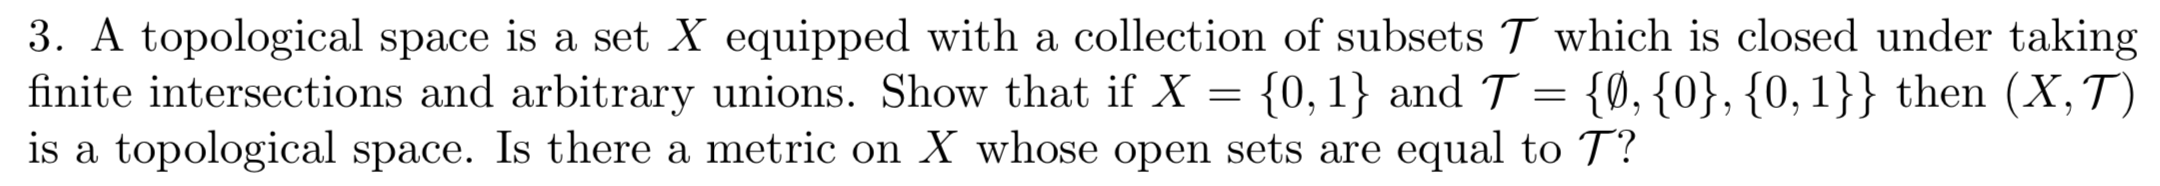
\includegraphics[width=400pt]{img/oxford-a2-2-3.png}
\end{mdframed}

\begin{proof}
  Let $X = \{0, 1\}$ and $\T = \{\emptyset, \{0\}, \{0, 1\}\}$.
  \begin{enumerate}
  \item $\emptyset \in \T$ and $X \in \T$ \checkmark
  \item {\bf Finite intersections}: \checkmark
    \begin{align*}
      \emptyset \cap \{0\}    &= \emptyset \in \T \\
      \emptyset \cap \{0, 1\} &= \emptyset \in \T \\
      \{0\}     \cap \{0, 1\} &= \{0\} \in \T
    \end{align*}
    Yes, it is closed under pairwise intersections so it must be closed under higher-order
    intersections. \red{hang on...why not just demand closure
      under pairwise intersections then?}
  \item {\bf Arbitrary unions}: \checkmark
    \begin{align*}
      \emptyset \cup \{0\}    &= \{0\}    \in \T \\
      \emptyset \cup \{0, 1\} &= \{0, 1\} \in \T \\
      \{0\}     \cup \{0, 1\} &= \{0, 1\} \in \T
    \end{align*}
    Yes, it is closed under pairwise unions so it must be closed under higher-order
    unions.
  \end{enumerate}
\end{proof}

\begin{proof}
  Suppose for a contradiction that $d$ is a metric on $X$ whose open sets are equal to $\T$.

  Then $\{0\} \in X$ is an open set under $d$.

  Therefore there exists $\epsilon > 0$ such that $B_d(0, \epsilon) = \{0\}$. Therefore
  $d(0, 1) = d(1, 0) > 0$.

  But then $\{1\}$ is an open set, since using the same $\epsilon$ we have
  $B_d(1, \epsilon) = \{1\}$. This contradicts the definition of $\T$.
\end{proof}

\red{So a singleton set containing an isolated point embedded in a metric space is open?}


\subsection{}



\begin{mdframed}
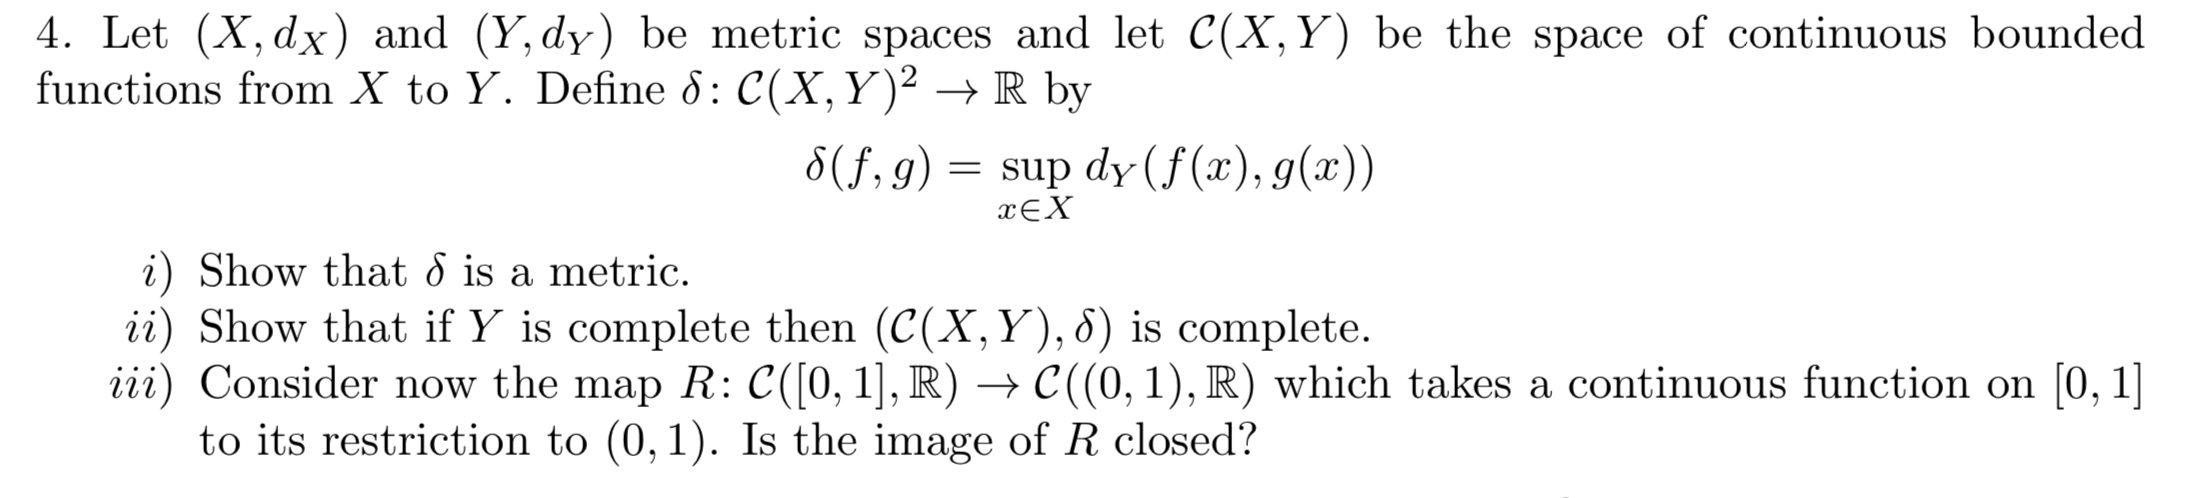
\includegraphics[width=400pt]{img/oxford-a2-2-4.png}
\end{mdframed}

\let\C\undefined
\newcommand{\C}{\mathcal{C}}

\begin{enumerate}[label=(\roman*)]
\item
  \begin{claim*}
    $\delta$ is a metric.
  \end{claim*}
  \begin{proof}~\\
    \begin{enumerate}
    \item {\bf Symmetry} \checkmark\\
      $d_Y$ is symmetric since it is a metric and therefore
      \begin{align*}
        \delta(f, g)
        = \sup_{x \in X} d_Y(f(x), g(x))
        = \sup_{x \in X} d_Y(g(x), f(x))
        = \delta(g, f).
      \end{align*}
    \item {\bf Positivity} \checkmark\\
      The codomain of $d_Y$ is $R_{\geq 0}$ since it is a metric and therefore
      $\sup_{a \in A} d_Y(a) \geq 0$ for all $A \subseteq Y^2$.
    \item {\bf Triangle inequality}\\
      Let $f, g, h \in \C(X, Y)$.

      We want
      \begin{align*}
        \delta(f, g) + \delta(g, h) &\leq \delta(f, h)\\
        \sup_{x \in X} d_Y(f(x), g(x)) +
        \sup_{x \in X} d_Y(g(x), h(x)) &\leq
        \sup_{x \in X} d_Y(f(x), h(x))
      \end{align*}

      We have
      \begin{align*}
        \delta(f, g) + \delta(g, h)
        &= \sup_{x \in X} d_Y(f(x), g(x)) +
           \sup_{x \in X} d_Y(g(x), h(x))
      \end{align*}
    \end{enumerate}
  \end{proof}
\item
  \newpage
  \begin{claim*}
    If $Y$ is complete then $\C(X, Y)$ is complete.
  \end{claim*}
  \begin{proof}~\\
    First, note that for all $f, g$ in $\C(X, Y)$ and for all $x \in X$ we have
    \begin{align*}
      d_Y(f(x), g(x)) \leq \delta(f, g).
    \end{align*}
    Suppose $Y$ is complete and let $(f_n)$ be a Cauchy sequence in $\C(X, Y)$.

    We want to show that $(f_n)$ converges in $\C(X, Y)$, and therefore that $\C(X, Y)$ is
    complete. The outline of our argument will be:
    \begin{enumerate}
    \item for all $x \in X$ the sequence $(f_n(x))$ in $Y$ is Cauchy;
    \item therefore such sequences converge in $Y$, since $Y$ is complete;
    \item therefore $(f_n)$ converges in $\C(X, Y)$, proving that $\C(X, Y)$ is complete.
    \end{enumerate}

    % For part (a), fix $\epsilon > 0$ and $x \in X$. We require an $N$ such that for all $m,n > N$
    % we have $d_Y(f_m(x), f_n(x)) < \epsilon$.

    For part (a), since $(f_n)$ is Cauchy in $\C(X, Y)$, we have for all $x \in X$
    \begin{align*}
      d_Y\(f_m(x), f_n(x)\) \leq \delta(f_m, f_n) \to 0 ~\text{as}~ m, n \to \infty.
    \end{align*}
    Therefore $(f_n(x))$ in $Y$ is Cauchy for all $x \in X$.

    % Since $(f_n)$ is Cauchy in $\C(X, Y)$ there exists an $N$ such that for all $m,n > N$ we have
    % $\delta(f_m, f_n) = \sup_{w\in X} d_Y(f_m(w), f_n(w)) < \epsilon$. Therefore for that same $N$
    % we have $d_Y(f_m(x), f_n(x)) < \epsilon$ for all $m,n > N$. Therefore $(f_n(x))$ is Cauchy and,
    % since $Y$ is complete, we have that $(f_n(x))$ converges, say to $L(x) \in Y$, for all
    % $x \in X$.

    For part (c), we need to show that there exists $f \in \C(X, Y)$ such that $f_n \to f$. We
    claim that $f(x) = \limn f_n(x)$ is such a function.

    Fix $\epsilon > 0$ and let $N$ be such that
    $d_Y\(f_m(x), f_n(x)\) \leq \delta(f_m, f_n) < \epsilon$ for all $x \in X$ and all $m, n > N$.

    Letting $m \to \infty$ we have $d_Y\(f(x), f_n(x)\) \leq \delta(f, f_n) < \epsilon$ for all
    $x \in X$ and all $m, n > N$. Thus we conclude $f_n \to f$, and also that $f - f_n$ is bounded.

    But the set of bounded functions $X \to Y$ is a vector space, and $f_n$ is bounded, so
    $f = f_n + (f - f_n)$ is bounded.

    Finally we must show $f$ is continuous.

    Note that the sequence $(f_n)$ (considered pointwise) converges uniformly to $f$ since for all
    $\epsilon > 0$ there exists $N$ such that for all $n > N$ we have
    $d_Y\(f_n(x), f(x)\) \leq \delta(f_n, f) < \epsilon$ for all $x \in X$. Therefore since the
    $f_n$ are continuous, we have that their limit $f$ is continuous.

  % % for all $\epsilon > 0$ there exists an $N$ such that for all $n > N$ we have
  % %   $\delta(f_n, f) < \epsilon$.



  %   To prove that $(f_n) \to f$, fix $\epsilon > 0$ and for all $x \in X$ define $M(x) \in \N$ to
  %   be the smallest natural number such that $d_Y(f_n(x), f(x)) < \epsilon$ for all $n > M(x)$.

  %   Set $N = \sup_{x \in X} M(x)$. Note that for all $n > N$ we have that
  %   \begin{align*}
  %     \delta(f_n, f) = \sup_{x\in X} d_Y(f_n(x), f(x)) < \epsilon,
  %   \end{align*}
  %   proving that $(f_n) \to f$.

  %   \newpage
  %   \red{Finally, we need to show that $f$ is continuous and bounded.}

  %   {\bf Continuity}:\\
  %   By definition, $f$ is continuous if $\lim_{x\to x_0} f(x) = f(x_0)$ for all $x_0 \in X$.

  %   {\bf Boundedness}:\\
  %   By definition, $f$ is bounded if there exists $r \geq 0$ such that $d_Y(f(x_1), f(x_2)) < r$
  %   for all $x_1, x_2 \in X$.

  %   So $f$ will be bounded if the set of pointwise limits $\{f(x)~|~x \in X\} \subseteq Y$ is
  %   bounded.
    Therefore if $(f_n)$ is Cauchy then it converges in $\C(X, Y)$, proving that $\C(X, Y)$ is
    complete.
  \end{proof}
\end{enumerate}



\end{document}
